\documentclass[a4paper,12pt]{article}
\usepackage{graphicx}
\usepackage{amsmath}
\usepackage[section]{placeins}
\usepackage{float}
\usepackage[scaled]{helvet}
\renewcommand\familydefault{\sfdefault} 
\usepackage[T1]{fontenc}
\usepackage{listings}
\usepackage{geometry}
\geometry{left=25mm, right=25mm, top=25mm, bottom=25mm}
\begin{document}
\title{REPORT FOR ASSIGNMENT 3\\CSE5CES}
\author{VU PHUC THANH TRAN\\ID: 18869804}
\maketitle{}
\newpage{}
\section*{Question 1}
\subsection*{How function get\_move() was implemented?}
Function get\_move() has 5 arguments which are:\\ \newline{}
\hspace*{1cm}+ A pointer which will point to variable (coordinate x) in function main().\\
\hspace*{1cm}+ A pointer which will point to variable (coordinate y) in function main().\\
\hspace*{1cm}+ A pointer which will point to variable (flag\_status) in function main().\\
\hspace*{1cm}+ Max value of coordinate x (value height in struct Game)\\
\hspace*{1cm}+ Max value of coordinate y (value of width in struct Game)\\
\newline{}
\noindent
- Inside function get\_move(), there is a do...while loop for receiving and validating input from users.\\
- In this do...while loop, a statement will be displayed for asking users to enter coordinates x (height), y (width) and flag (0/1) by using function scanf().\\
- After using scanf(), a code statement is used for cleaning keyboard buffer. That will make sure that other functions scanf() will not operate in wrong way.\\
- After receiving those inputs from users, they will be validated to make sure that there is any bad effects on the others part of the program.\\
\newline{}
- A variable named `check` are created to get return result from function scanf()\\
\hspace*{1cm}+ IF check is equal to zero, THEN that means scan() can not get any value from keyboard buffer and storing to the variable.\\
- There are three conditions for do...while loop. If one or more than one of them are fail, then the program will start to ask users about inputs again. If all of them are successful, then the program will get out of loop and return values for three variables in function main(): x, y, flag\_status via pointers.\\
\newline{}
Condition 1: IF check is equal to zero\\
OR\\
Condition 2: IF x (input) or y (input) are larger than max value of x and y\\
OR\\
Condition 3: IF flag (input) is not equal to zero and flag (input) is not equal to one\\
\newline{}
\subsection*{Why get\_move() was implemented that way?}
- Do...while loop was used because it does code block inside first then check conditions at the end of the loop. Therefore, all code block for asking users, receiving inputs and validating could be placed inside the loop and will be displayed again if users enter invalid input.\\
- After using scanf(), there need to be a code statement for cleaning buffer. Because, sometimes, scanf() just takes part of keyboard buffer or does not take any thing and leaving all data in buffer. Therefore, cleaning buffer will help to avoid unpredicted effects on the program.\\
- 3 of 5 arguments (get\_move()) are pointers which point to those variables in function main(). This assignment requires to get and return three variables to function main(), so, pointer need to be used.\\
\section*{Question 2}
\subsection*{How step 6 and 7 in function main were implemented?}
- First of all, to create a two dimensions array for storing mine\_board, there need to be a pointer with two stars (**) (pointer which points to another pointer). In the program, a pointer with 2 stars was declared.\\
\begin{lstlisting}
struct Location** mine_board;
\end{lstlisting}
- First pointer will point to an array which is assigned by function malloc() with data type is struct Location**. The length of this array is equal to height of the game board + 2 (input from users).\\
\begin{lstlisting}
mine_board = (struct Location**)malloc((game.height + 2) * 
sizeof(struct Location));
\end{lstlisting}
- Each element in that array is also a pointer, that pointer will pointer to an array assigned by function malloc() with data type is struct Location*. Then, a loop can be used for assigning each element in first array to an array (by function malloc()). The length of each array is equal to width of game board + 2 (input from users).\\
\begin{lstlisting}
for(i = 0; i < (game.height + 2); i++)
	{
		mine_board[i] = (struct Location*)malloc((game.width + 2) * 
		sizeof(struct Location));
		if(NULL == mine_board[i])
		{
			printf("Error of malloc() function\n");
			return 1;
		}
	}
\end{lstlisting}
- After each time using function malloc(), an if...else will be used for comparing the variable which was assigned by malloc() with NULL value. If that variable is equal to NULL, the program will exit and displaying an error statement.\\
- Finally, a two dimension array was created.\\
\subsection*{Why are step 6 and 7 implemented that way?}
- Game field need to be created after receiving height and width from user's need. Hence, malloc() will be used to create array which is based on user's need.\\
- First, an array which presents for height of game board will be created by malloc(). \\
- Then for each row, malloc() need to be operated again to create array (width)(column) for each row. This part will be put on a loop.\\ 
- When using malloc() for creating arrays, two more rows and two more columns were added. Thus, these rows and column will be used for borders around game field.\\
\section*{How function make\_move() run?}
There are 4 arguments in function make\_move():\\
\hspace*{1cm}1 - a variable with data type struct Game\\
\hspace*{1cm}2 - a pointers with two starts which will points to variable mine\_board in function main()\\
\hspace*{1cm}3 - value of coordinate x\\
\hspace*{1cm}4 - value of coordinate y\\
\newline{}
- When make\_move() is called, value of game (struct Game) in function main will be passed to first argument. Then, value of coordinate x and value of coordinate y in function main will be passed to third and fourth arguments as well. The pointer (second argument) will point to variable mine\_board in function main().\\
- Function make\_move() will take coordinate x, y and setting REVEALED bit to 1 at this position.\\
- Checking if there is a mine of this location or not\\
\hspace{1cm}+ Yes: set statusOfPlayer to zero (gameover)\\
\hspace{1cm}+ No\\
\hspace{2cm}. Checking if there is a flag, then remove that flag.\\
\hspace{2cm}. Checking if value of this location is equal to zero, then call function uncover\_zeros().\\
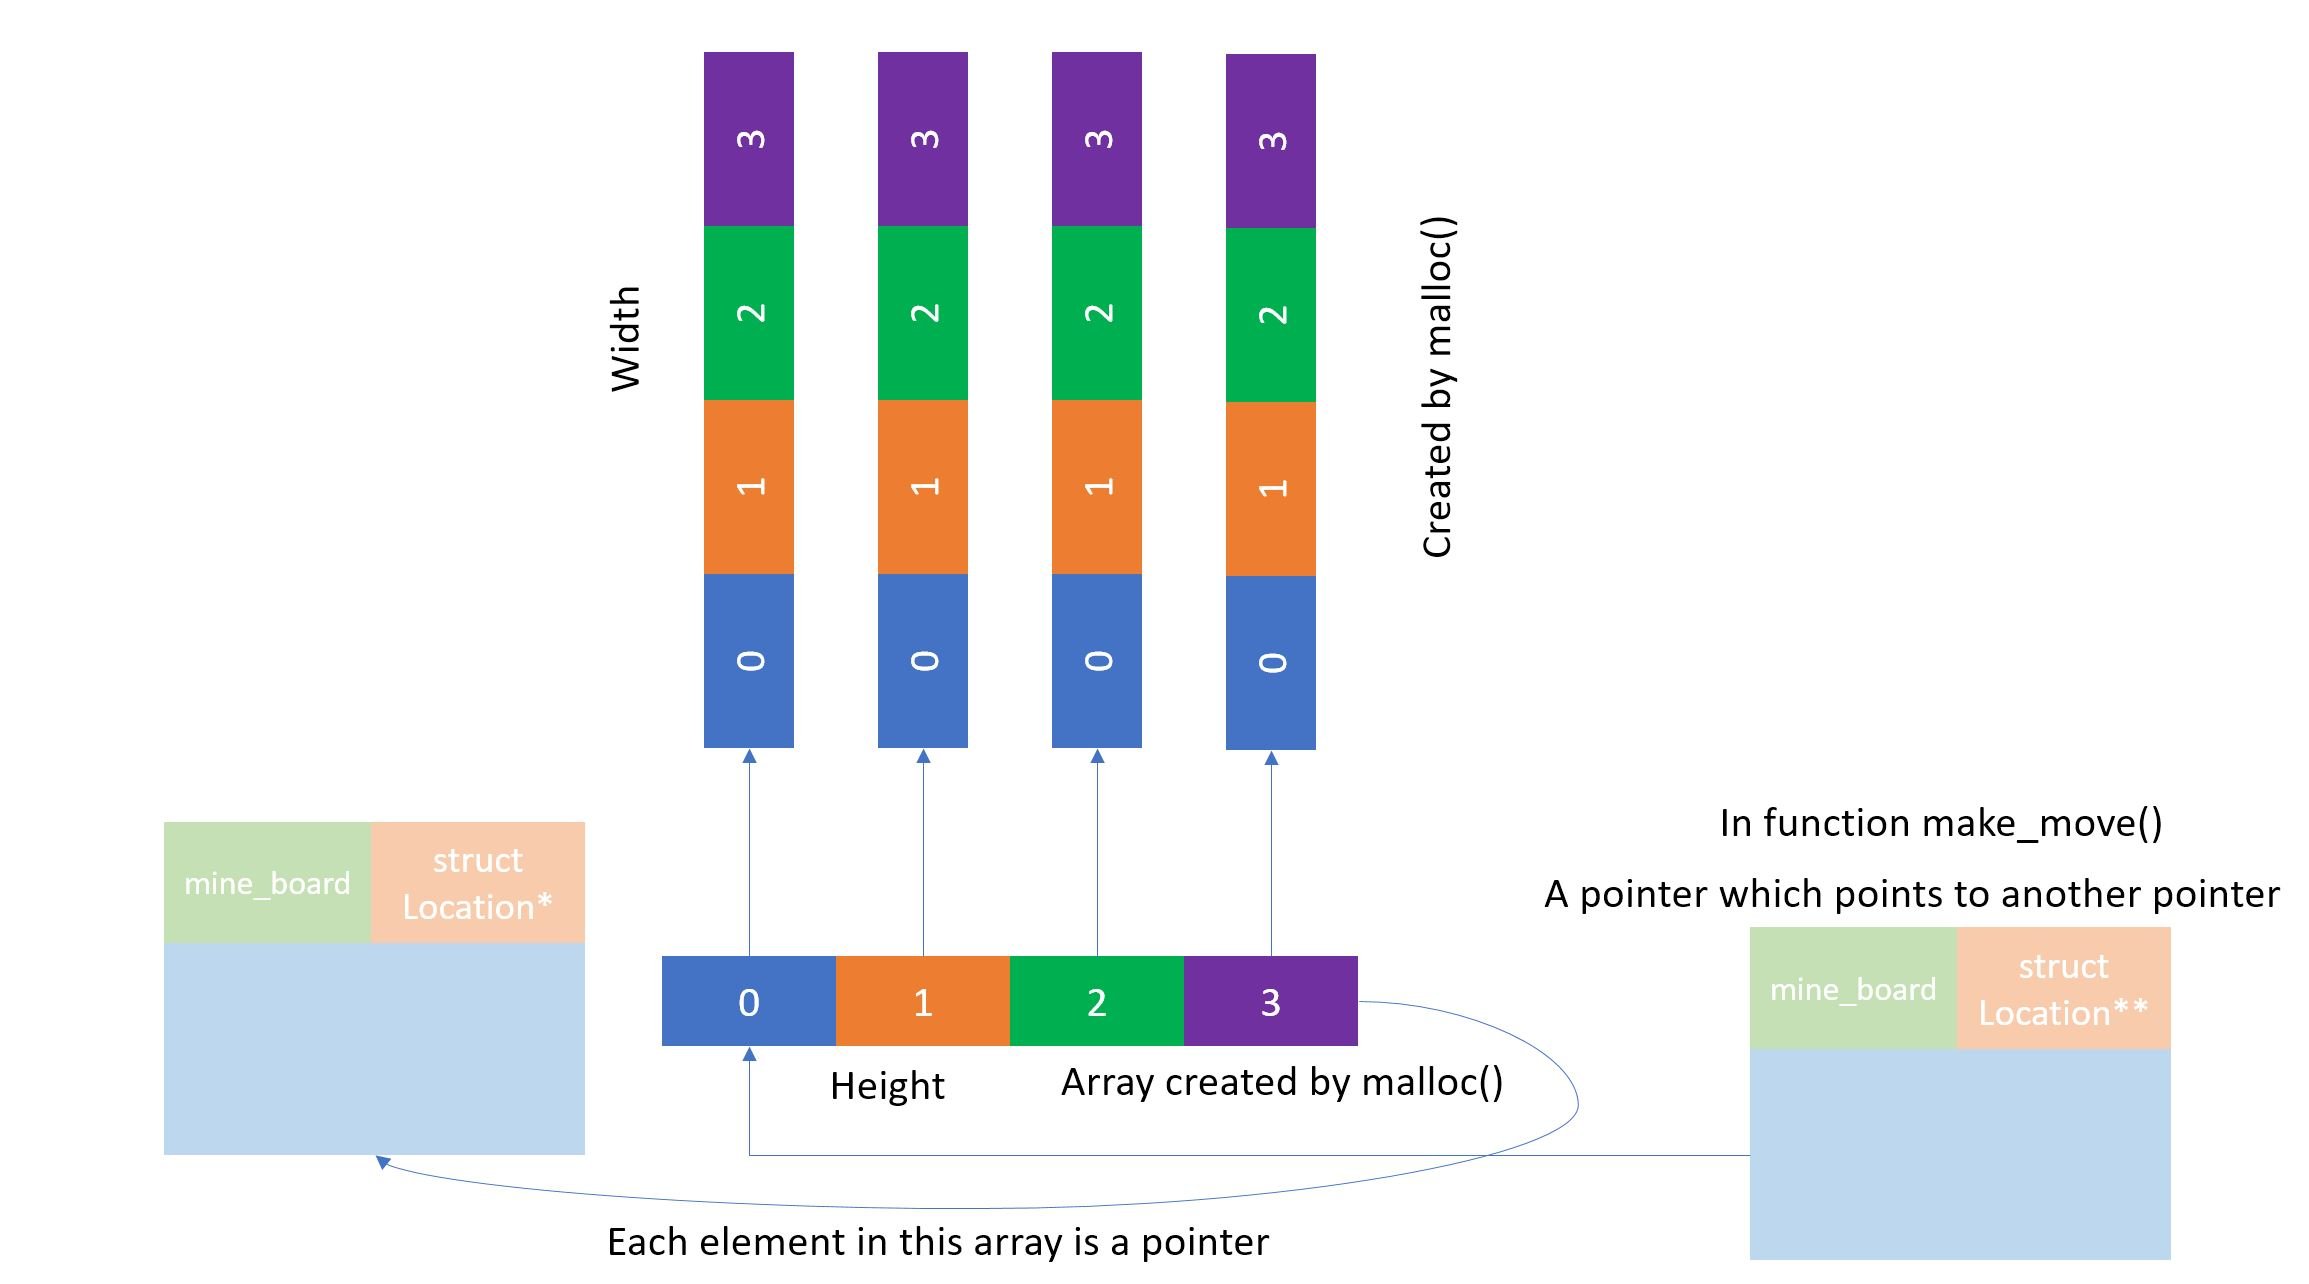
\includegraphics[width=\textwidth]{Capture.JPG}
\end{document}